\documentclass[conference]{IEEEtran}

\usepackage[T1]{fontenc}
\usepackage[utf8]{inputenc}
\usepackage{cite}
\usepackage{amsmath,amssymb}
\usepackage{graphicx}
\usepackage{booktabs}
\usepackage{multirow}
\usepackage{array}
\usepackage{hyperref}
\usepackage{xcolor}
\usepackage{float}

\hypersetup{
    colorlinks=true,
    linkcolor=blue,
    citecolor=blue,
    urlcolor=blue
}

\title{Crop Recommendation Using Soil Nutrients and Weather Data: \\A Comparative Machine Learning Study}

\author{%
\begin{tabular}{cc}
  \begin{tabular}[t]{c}
    \textbf{Vidhan Sachdeva}\\[2pt]
    Reg. No.: 240968030\\
    Roll No.: 07\\[2pt]
    \textit{Manipal Institute of Technology, Manipal}\\
    {\small vidhan.mitmpl2024@learner.manipal.edu}
  \end{tabular}
  &
  \begin{tabular}[t]{c}
    \textbf{Rohan Rajesh Bangera}\\[2pt]
    Reg. No.: 240968027\\
    Roll No.: 06\\[2pt]
    \textit{Manipal Institute of Technology, Manipal}\\
    {\small rohan.mitmpl2024@learner.manipal.edu}
  \end{tabular}
  \\[2.5em]
  \begin{tabular}[t]{c}
    \textbf{Mishal Muhammed}\\[2pt]
    Reg. No.: 240968192\\
    Roll No.: 20\\[2pt]
    \textit{Manipal Institute of Technology, Manipal}\\
    {\small mishal.mitmpl2024@learner.manipal.edu}
  \end{tabular}
  &
  \begin{tabular}[t]{c}
    \textbf{Amish Kishore Shetty}\\[2pt]
    Reg. No.: 240968094\\
    Roll No.: 14\\[2pt]
    \textit{Manipal Institute of Technology, Manipal}\\
    {\small amish.mitmpl2024@learner.manipal.edu}
  \end{tabular}
  \\[2.5em]
  \begin{tabular}[t]{c}
    \textbf{Isheet Bohra}\\[2pt]
    Reg. No.: 240968035\\
    Roll No.: 08\\[2pt]
    \textit{Manipal Institute of Technology, Manipal}\\
    {\small isheet.mitmpl2024@learner.manipal.edu}
  \end{tabular}
  &
  \begin{tabular}[t]{c}
    \textbf{C Rohan Sai}\\[2pt]
    Reg. No.: 240968158\\
    Roll No.: 17\\[2pt]
    \textit{Manipal Institute of Technology, Manipal}\\
    {\small rohan1.mitmpl2024@learner.manipal.edu}
  \end{tabular}
\end{tabular}
}

\begin{document}

\maketitle

\begin{abstract}
Precision agriculture benefits from predictive systems that can translate soil and weather measurements into actionable crop recommendations. This paper presents an end-to-end machine learning pipeline for multi-class crop recommendation using seven agronomic features: nitrogen, phosphorus, potassium, temperature, humidity, pH, and rainfall. The study follows a research-style methodology including statistical analysis, controlled missing-value benchmarking, outlier analysis, feature engineering, dimensionality reduction experiments, hyperparameter tuning, cross-validation, ensemble learning, and model interpretability. Twelve candidate models were compared, including classical machine learning methods, gradient boosting methods, neural networks, and ensemble meta-models. On the evaluated dataset of 2,200 samples across 22 balanced crop classes, the Soft Voting ensemble achieved the best overall performance with a test accuracy of 0.9932 and a macro-F1 score of 0.9932. Additional analysis using SHAP, permutation importance, and significance tests supports the robustness and interpretability of the selected model. The resulting system provides a strong baseline for deployment-oriented crop recommendation and future region-specific agricultural decision support.
\end{abstract}

\begin{IEEEkeywords}
crop recommendation, precision agriculture, ensemble learning, machine learning, interpretability, IEEE
\end{IEEEkeywords}

\section{Introduction}
Agriculture remains highly dependent on environmental conditions such as soil fertility, nutrient balance, moisture availability, and climate variability. In many practical settings, crop selection still relies on local heuristics or experience-driven choices, which may not fully exploit the growing availability of agricultural data. Machine learning offers a promising route to improve such decisions by mapping soil and weather variables to crop suitability classes \cite{klompenburg2020,liakos2018}.

The objective of this work is to design a rigorous crop recommendation pipeline rather than a minimal predictive script. In addition to prediction accuracy, the study emphasizes preprocessing comparisons, statistical diagnostics, model benchmarking, bias-variance analysis, and interpretability. The resulting workflow aims to be useful both as an academic artifact and as a foundation for a deployable recommendation tool.

The motivation behind this study is practical as well as methodological. From a practical point of view, recommending a suitable crop from local soil nutrients and weather values can improve resource allocation, reduce failed planting choices, and support more informed agricultural planning. From a methodological point of view, agricultural datasets are often analyzed using a single model or a small preprocessing pipeline, which can hide how much performance depends on imputation choices, scaling, feature interactions, or model selection. This work therefore treats crop recommendation as a complete comparative study.

\section{Related Work}
Crop yield and crop recommendation systems have been widely studied using both classical machine learning and deep learning techniques. Systematic literature reviews show strong performance from ensemble methods such as Random Forest, Gradient Boosting, and neural architectures when agricultural variables are sufficiently informative \cite{klompenburg2020}. Random forests have been used effectively for regional and global agricultural prediction tasks \cite{jeong2016}, while deep neural networks have also demonstrated competitive performance for crop-related prediction tasks \cite{khaki2019}. Broader surveys of machine learning in agriculture highlight the importance of data quality, model interpretability, and domain-specific feature engineering \cite{liakos2018}.

\section{Dataset and Problem Formulation}
The task is formulated as a multi-class classification problem. Each sample contains seven numerical input features:
\begin{itemize}
    \item Nitrogen (N)
    \item Phosphorus (P)
    \item Potassium (K)
    \item Temperature
    \item Humidity
    \item pH
    \item Rainfall
\end{itemize}

The target variable is the crop label. The dataset used in this project contains 2,200 samples and 22 crop classes, with 100 samples per class. Because the classes are perfectly balanced, macro-averaged metrics are especially informative and were emphasized during evaluation.

Let the input vector for each sample be represented as
\begin{equation}
\mathbf{x} = [N, P, K, T, H, pH, R]^\top
\end{equation}
where $T$ denotes temperature, $H$ denotes humidity, and $R$ denotes rainfall. The task is to learn a mapping
\begin{equation}
f : \mathbf{x} \rightarrow y
\end{equation}
where $y$ belongs to one of 22 crop classes. Since the target has more than two classes and the dataset is balanced, macro-averaged precision, recall, and F1-score were prioritized along with accuracy.

\section{Methodology}
\subsection{Statistical Preprocessing}
Although the original dataset contained no missing values, imputation methods were still compared through controlled synthetic masking to assess robustness under incomplete input conditions. Five imputation strategies were studied:
\begin{itemize}
    \item Mean imputation
    \item Median imputation
    \item KNN imputation
    \item Iterative regression-based imputation
    \item EM-style Gaussian imputation
\end{itemize}

Their impact was assessed using reconstruction RMSE and downstream macro-F1. In other words, the study did not assume that a mathematically good imputer would automatically produce the best classification performance. Instead, each imputation strategy was judged using both numerical reconstruction quality and its influence on final predictive accuracy. Friedman tests were used to compare methods statistically across repeated masking experiments.

Outliers were analyzed using:
\begin{itemize}
    \item Z-score thresholding
    \item Interquartile range (IQR) analysis
    \item Mahalanobis distance for multivariate outliers
\end{itemize}

Correlation matrices, covariance analysis, ANOVA, Kruskal-Wallis testing, and variance inflation factor (VIF) diagnostics were computed to inspect linear relationships and multicollinearity. Pearson correlation was used to examine linear dependence between continuous variables, while Spearman correlation was used to capture monotonic relationships that may not be strictly linear. ANOVA and Kruskal-Wallis tests were included to verify whether individual features differed significantly across crop classes.

\subsection{Feature Engineering and Transformation}
Domain-inspired features were added to enrich the representation, including:
\begin{itemize}
    \item total NPK sum
    \item nutrient balance
    \item rainfall-to-temperature ratio
    \item humidity-temperature interaction
    \item pH distance from neutrality
    \item nutrient density
    \item climate stress index
\end{itemize}

These transformations were introduced to make the feature space more expressive from an agronomic standpoint. For example, total NPK sum provides a simple measure of overall nutrient availability, while rainfall-to-temperature ratio and climate stress index help capture environmental interactions rather than isolated measurements. Scaling strategies compared included StandardScaler, MinMaxScaler, and RobustScaler. Dimensionality reduction experiments were performed with PCA and LDA. Polynomial interaction features and power transformations were also considered during model tuning.

\subsection{Models Evaluated}
The following models were tuned and evaluated:
\begin{itemize}
    \item Logistic Regression
    \item Decision Tree
    \item Random Forest
    \item K-Nearest Neighbors
    \item Gaussian Naive Bayes
    \item Support Vector Machine
    \item Gradient Boosting
    \item XGBoost
    \item LightGBM
    \item Multi-Layer Perceptron
    \item Soft Voting ensemble
    \item Stacking ensemble
\end{itemize}

Hyperparameter tuning was performed using GridSearchCV or RandomizedSearchCV depending on model complexity. Simpler models such as Logistic Regression and KNN were tuned using structured grid search, while more complex models such as Random Forest, XGBoost, LightGBM, and MLP were tuned using randomized search over a bounded but meaningful parameter space. Evaluation used stratified cross-validation and a final hold-out test split.

The study also included two ensemble approaches. Soft Voting combined class probabilities from the strongest tuned base models, while Stacking used the outputs of top-performing learners as inputs to a meta-classifier. This design was intended to test whether combining complementary decision boundaries could produce better generalization than any single classifier alone.

\subsection{Evaluation Metrics}
Model performance was evaluated using accuracy, precision, recall, and macro-F1 score. For a multi-class setting, these metrics were computed class-wise and then macro-averaged to ensure that each crop class contributed equally. Accuracy is defined as
\begin{equation}
\text{Accuracy} = \frac{TP + TN}{TP + TN + FP + FN}
\end{equation}
where $TP$, $TN$, $FP$, and $FN$ denote true positives, true negatives, false positives, and false negatives, respectively.

Precision and recall are defined as
\begin{equation}
\text{Precision} = \frac{TP}{TP + FP}
\end{equation}
\begin{equation}
\text{Recall} = \frac{TP}{TP + FN}
\end{equation}

The F1-score is the harmonic mean of precision and recall:
\begin{equation}
F1 = \frac{2 \cdot \text{Precision} \cdot \text{Recall}}{\text{Precision} + \text{Recall}}
\end{equation}

For balanced multi-class classification, macro-F1 is especially useful and is defined as
\begin{equation}
F1_{\text{macro}} = \frac{1}{K}\sum_{i=1}^{K} F1_i
\end{equation}
where $K$ is the number of crop classes and $F1_i$ is the class-wise F1-score for class $i$.

To assess overfitting, a simple bias-variance gap was also computed as the difference between mean training accuracy and mean validation accuracy:
\begin{equation}
\Delta_{bv} = \text{Train Accuracy}_{mean} - \text{Validation Accuracy}_{mean}
\end{equation}

\subsection{Hypothesis Testing}
Statistical hypothesis testing was used at two levels. First, during preprocessing, the null hypothesis for imputation comparison stated that all imputation methods have equivalent performance under repeated masking experiments. Because multiple imputers were compared across repeated trials, a Friedman test was used:
\begin{equation}
H_0: \mu_{\text{mean}} = \mu_{\text{median}} = \mu_{\text{knn}} = \mu_{\text{iterative}} = \mu_{\text{em}}
\end{equation}
against the alternative that at least one method differs significantly.

Second, model-level comparisons were performed using paired tests on fold-wise macro-F1 scores. For two models $A$ and $B$, the null hypothesis was:
\begin{equation}
H_0: \mu_{F1}^{(A)} = \mu_{F1}^{(B)}
\end{equation}
and the alternative hypothesis was
\begin{equation}
H_1: \mu_{F1}^{(A)} \neq \mu_{F1}^{(B)}
\end{equation}

Paired $t$-tests and Wilcoxon signed-rank tests were used to compare the best model against other candidates. This combination was chosen to provide both a parametric and a non-parametric perspective on score differences.

\section{Results and Discussion}
\subsection{Preprocessing Findings}
The best imputation method under synthetic missingness was KNN imputation. The Friedman test indicated statistically significant differences between imputation strategies for both reconstruction error and downstream macro-F1, with p-values of 0.000771849 and 0.00656719 respectively. This suggests that even when missingness is artificially introduced, preprocessing choices can materially change downstream classification quality. In baseline scaling experiments, the best scaler-model combination was RobustScaler with MLP, yielding a macro-F1 of 0.9877. For dimensionality reduction, LDA gave the strongest baseline result with macro-F1 of 0.9840.

\begin{figure}[H]
    \centering
    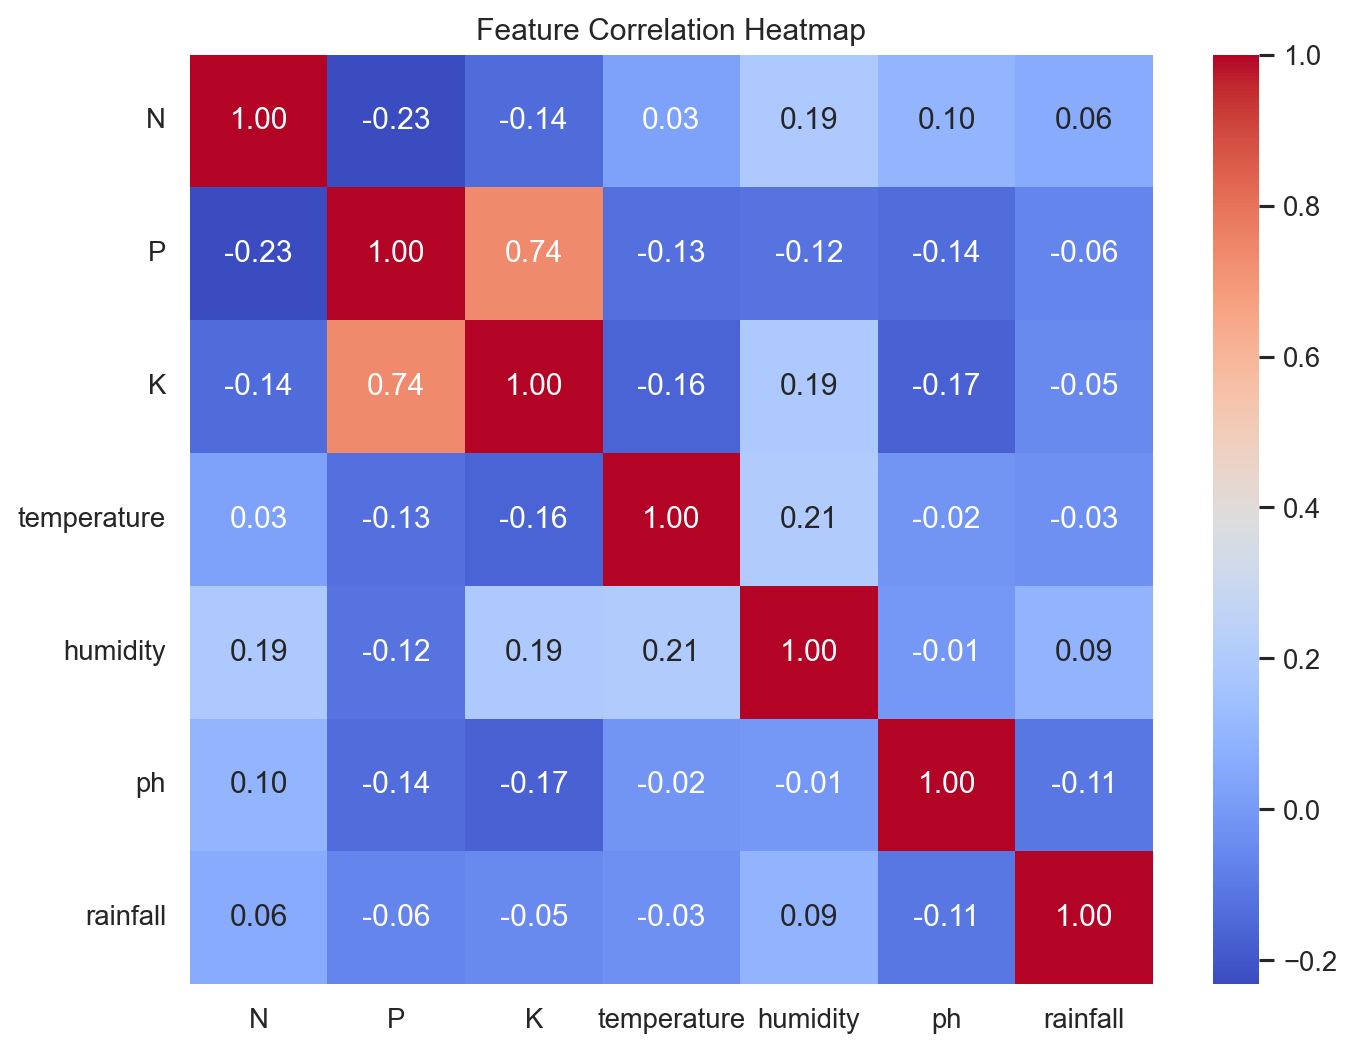
\includegraphics[width=0.9\linewidth]{figures/correlation_heatmap.png}
    \caption{Correlation heatmap of the seven core agronomic features.}
    \label{fig:corr}
\end{figure}

\begin{figure}[H]
    \centering
    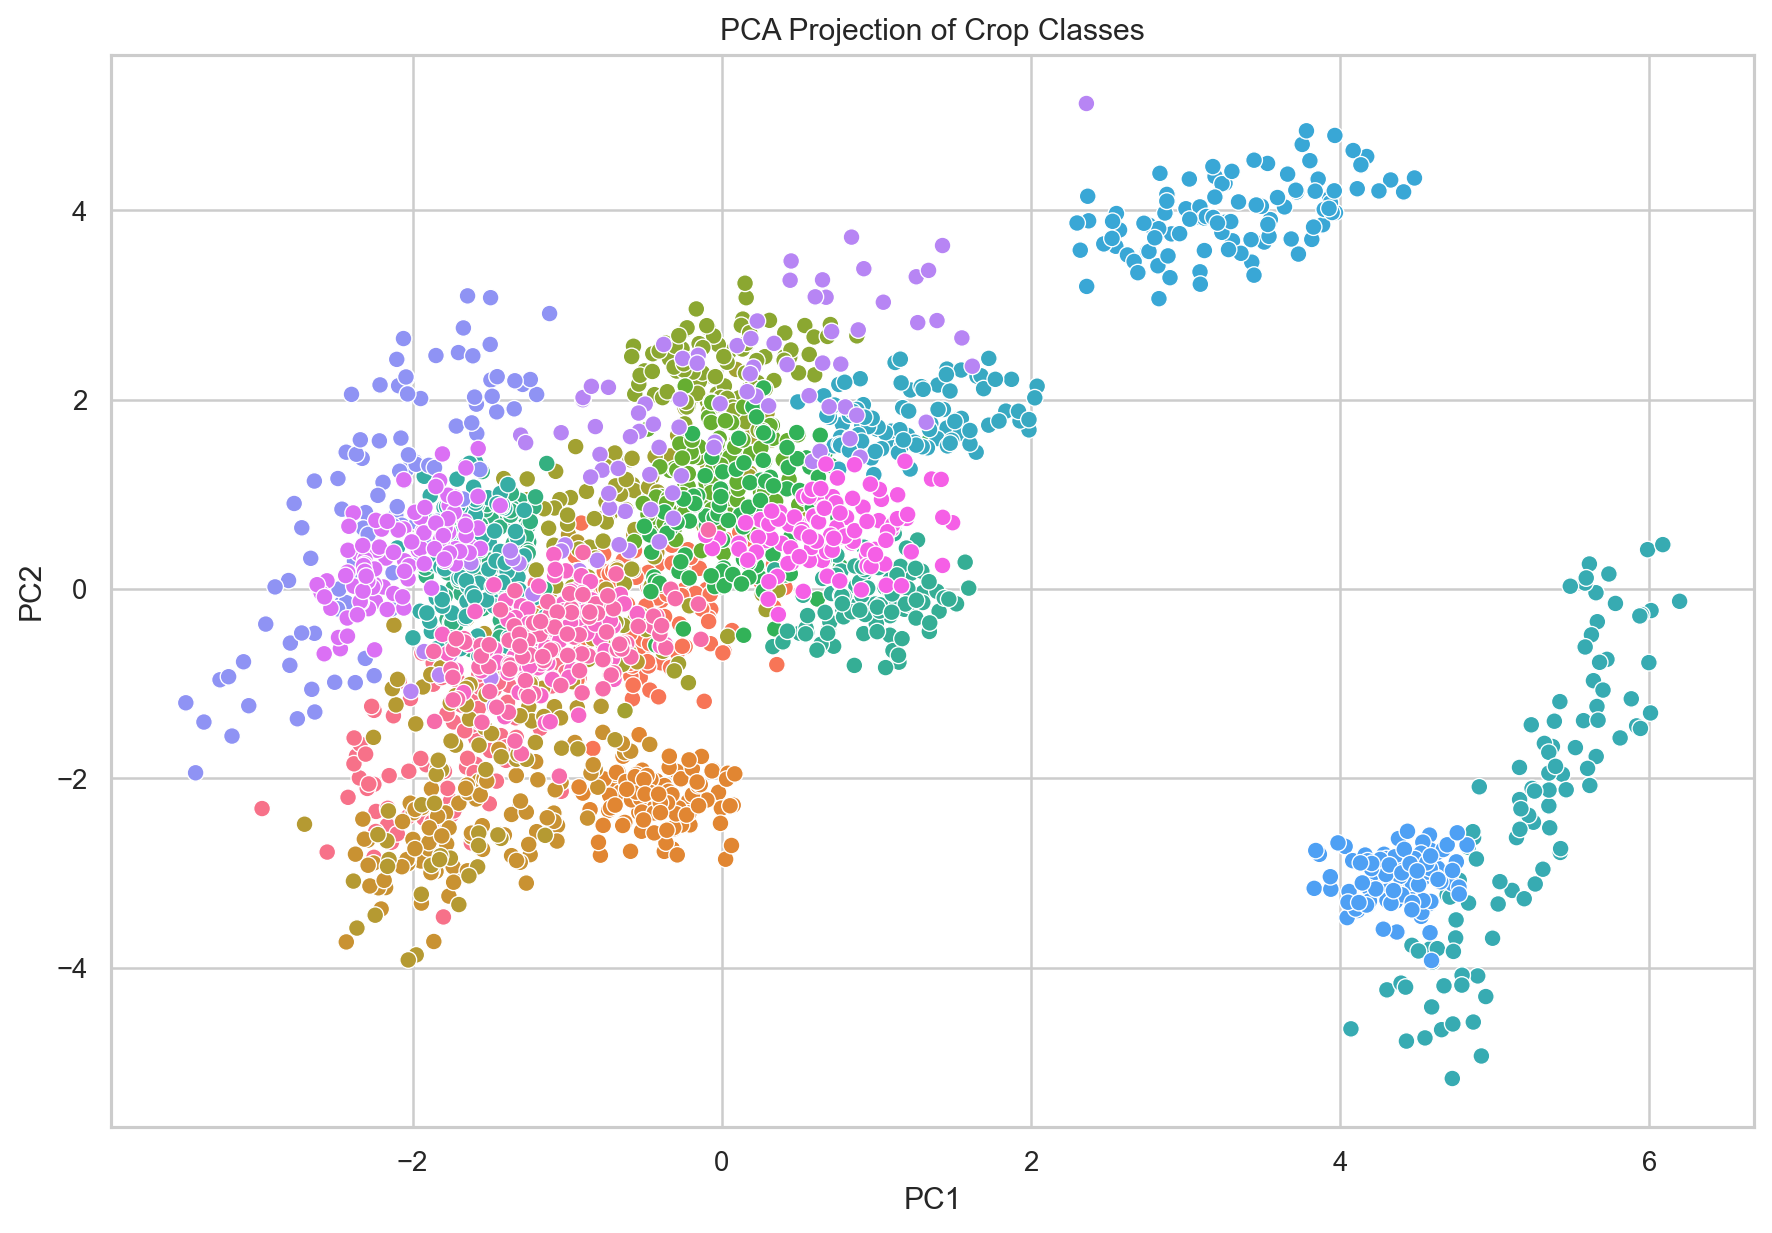
\includegraphics[width=0.9\linewidth]{figures/pca_scatter.png}
    \caption{PCA projection showing class separation structure in the crop dataset.}
    \label{fig:pca}
\end{figure}

\subsection{Model Comparison}
Table~\ref{tab:leaderboard} summarizes representative model results. Several models achieved very high accuracy, but the final Soft Voting ensemble was selected because it provided the strongest balance between test performance and cross-validation stability. It is important to note that LightGBM, Random Forest, GaussianNB, and Stacking all performed competitively, which indicates that the dataset contains a strong underlying signal that is recoverable by several learning paradigms. Nevertheless, Soft Voting was retained because it matched the best hold-out metrics while also maintaining very strong cross-validation behavior.

\begin{table}[H]
\centering
\caption{Top model comparison on the crop recommendation dataset}
\label{tab:leaderboard}
\begin{tabular}{lccc}
\toprule
Model & CV Macro-F1 & Test Accuracy & Test Macro-F1 \\
\midrule
SoftVoting & 0.9909 & 0.9932 & 0.9932 \\
GaussianNB & 0.9909 & 0.9932 & 0.9932 \\
Stacking & 0.9904 & 0.9932 & 0.9932 \\
RandomForest & 0.9903 & 0.9932 & 0.9932 \\
LightGBM & 0.9841 & 0.9932 & 0.9932 \\
XGBoost & 0.9864 & 0.9909 & 0.9908 \\
SVM & 0.9829 & 0.9886 & 0.9886 \\
DecisionTree & 0.9720 & 0.9682 & 0.9681 \\
\bottomrule
\end{tabular}
\end{table}

\begin{table}[H]
\centering
\caption{Paired significance tests using SoftVoting as reference}
\label{tab:significance}
\begin{tabular}{lcc}
\toprule
Comparison Model & Paired $t$-test $p$ & Wilcoxon $p$ \\
\midrule
GaussianNB & 0.9858 & 1.0000 \\
Stacking & 0.7544 & 1.0000 \\
RandomForest & 0.8400 & 1.0000 \\
LightGBM & 0.0781 & 0.2500 \\
LogisticRegression & 0.0001 & 0.2500 \\
GradientBoosting & 0.0107 & 0.2500 \\
XGBoost & 0.3867 & 0.5000 \\
MLP & 0.0708 & 0.2500 \\
SVM & 0.0319 & 0.2500 \\
KNN & 0.0074 & 0.2500 \\
DecisionTree & 0.0525 & 0.2500 \\
\bottomrule
\end{tabular}
\end{table}

\begin{figure}[H]
    \centering
    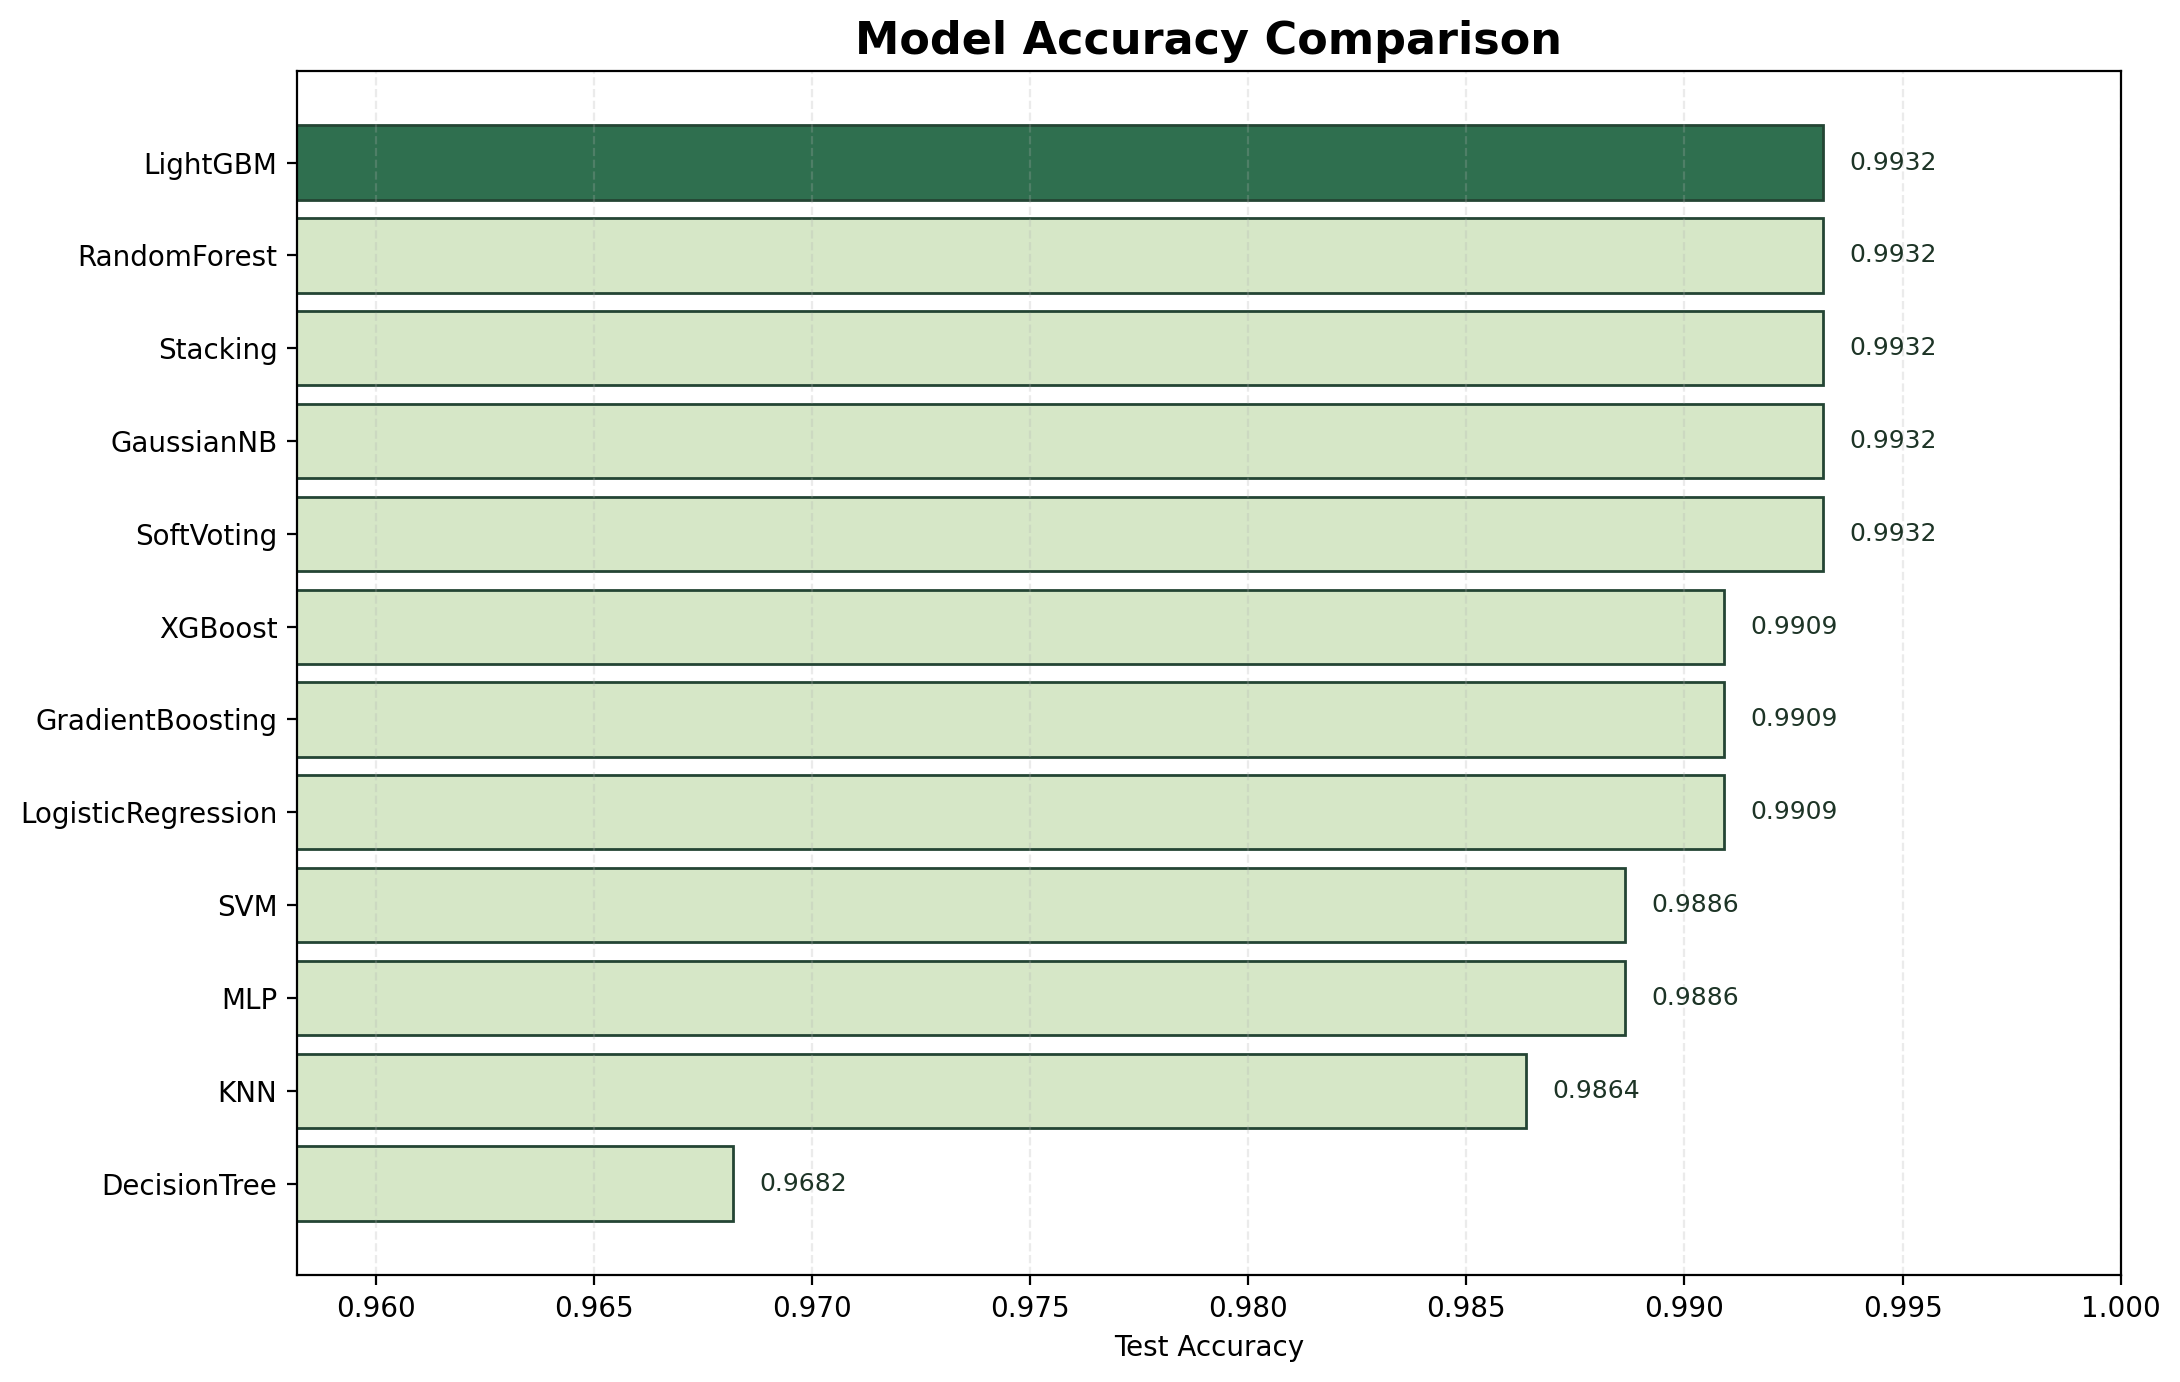
\includegraphics[width=0.95\linewidth]{figures/model_accuracy_comparison.png}
    \caption{Comparison of test accuracy across all evaluated models.}
    \label{fig:acccompare}
\end{figure}

The selected Soft Voting model achieved:
\begin{itemize}
    \item Test accuracy: 0.9932
    \item Test macro-F1: 0.9932
    \item Balanced accuracy: 0.9932
    \item Top-3 accuracy: 1.0000
    \item Cross-validation macro-F1: 0.9909
\end{itemize}

The bias-variance gap for Soft Voting was only 0.0034, suggesting no strong evidence of overfitting on the evaluated dataset. The closeness between the cross-validation macro-F1 and the final test macro-F1 also supports this conclusion. Paired significance tests showed that the best ensemble outperformed weaker baselines such as Logistic Regression and KNN more clearly than near-tied high performers such as GaussianNB or RandomForest. This indicates that the advantage of the final model is real but relatively small against the very strongest competitors.

The hypothesis testing results in Table~\ref{tab:significance} support this interpretation. The Soft Voting ensemble was not significantly different from the strongest near-tied contenders such as GaussianNB, RandomForest, or Stacking under the small cross-validation sample size, but it showed clearer separation from weaker baselines such as Logistic Regression, Gradient Boosting, SVM, and KNN. This pattern suggests that the final model should be interpreted as the most reliable aggregate performer rather than the only strong model in the study.

\begin{figure}[H]
    \centering
    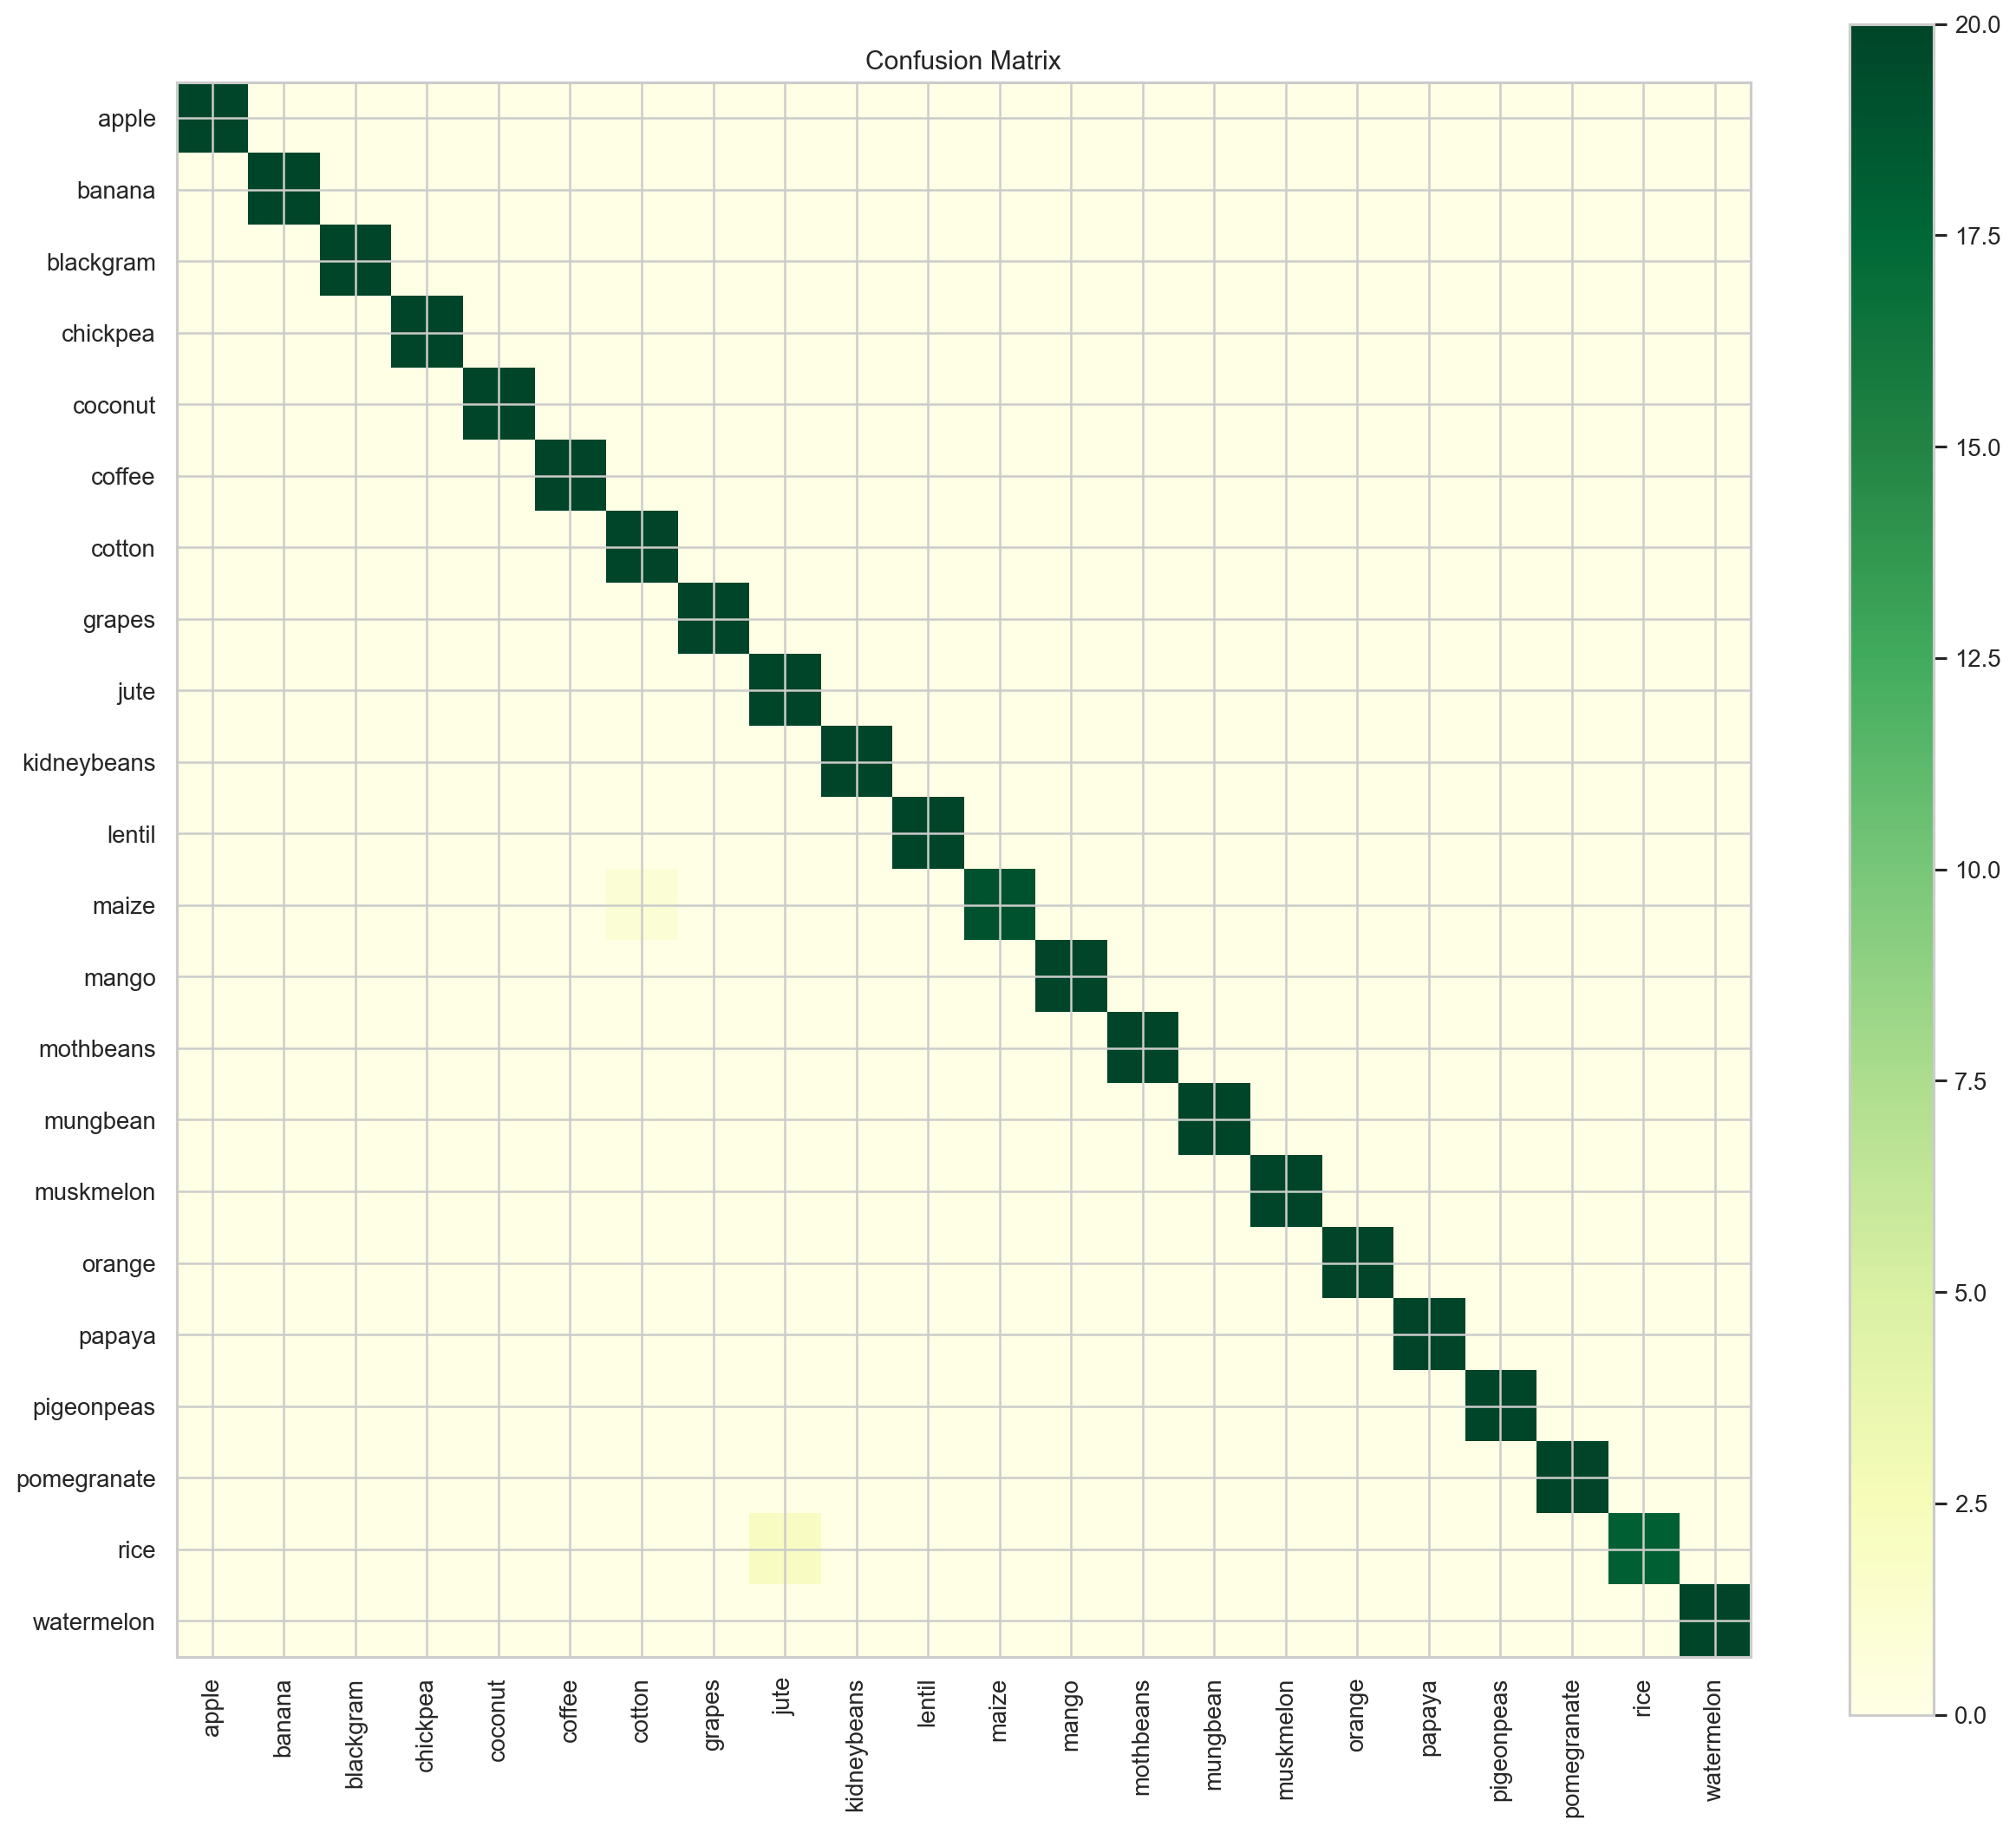
\includegraphics[width=0.9\linewidth]{figures/confusion_matrix.png}
    \caption{Confusion matrix of the selected final model on the test split.}
    \label{fig:cm}
\end{figure}

\subsection{Interpretability}
To reduce the black-box nature of the final system, the study included permutation importance, SHAP analysis, and LIME local explanation. The SHAP summary in Fig.~\ref{fig:shap} suggests that nutrient concentrations, rainfall, and pH-related patterns remain among the most influential signals across predictions. This is consistent with agricultural intuition, since nutrient availability and moisture-related variables strongly influence whether a crop can be sustained under local conditions.

Interpretability was included for two reasons. First, agricultural recommendation systems are more useful when they support explanation rather than only outputting a label. Second, when several high-performing models exist, explanation tools provide an additional way to verify that predictions are based on meaningful agronomic features rather than unstable artifacts in the dataset.

\begin{figure}[H]
    \centering
    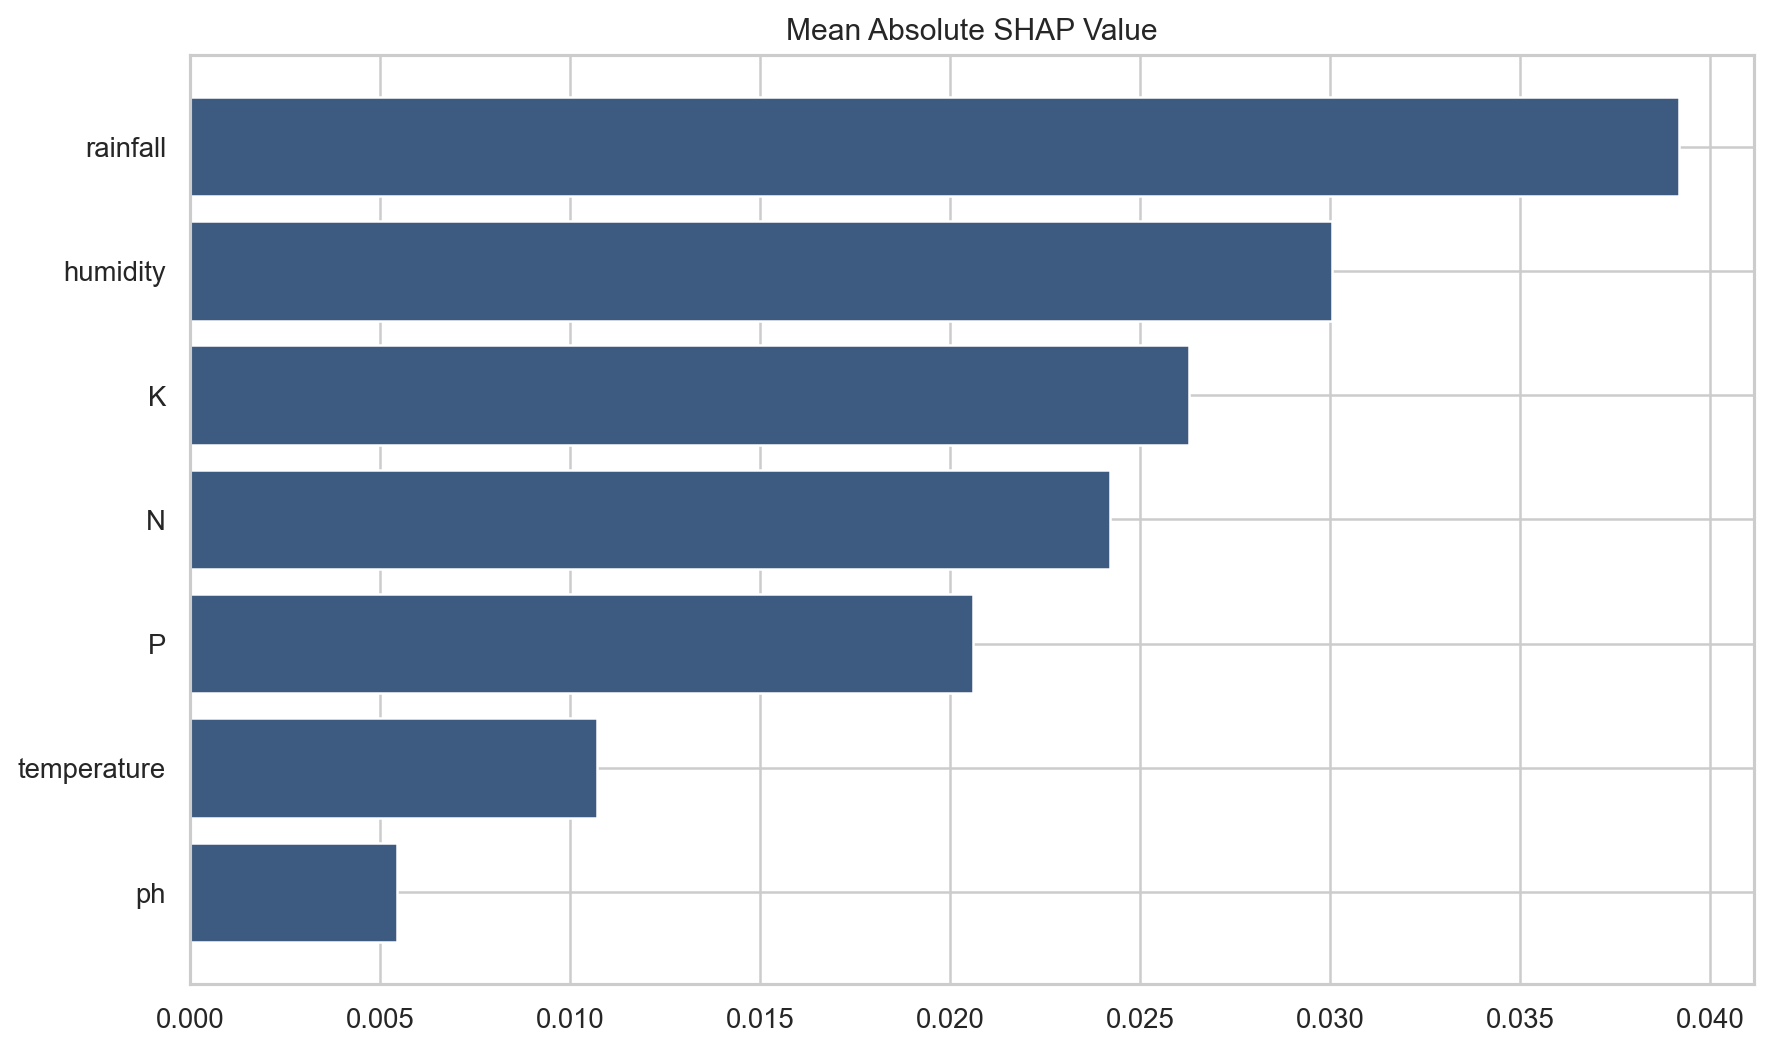
\includegraphics[width=0.85\linewidth]{figures/shap_global_importance.png}
    \caption{Global feature importance estimated using SHAP values.}
    \label{fig:shap}
\end{figure}

\section{Conclusion}
This paper presented a complete IEEE-style machine learning study for crop recommendation using soil and weather measurements. The contribution lies not only in high predictive performance but also in the rigor of the comparative methodology: imputation benchmarking, outlier analysis, statistical diagnostics, model tuning, ensemble comparison, and interpretability. The final Soft Voting ensemble achieved the best overall balance of accuracy, macro-F1, and generalization stability on the evaluated dataset.

Overall, the study demonstrates that careful preprocessing and model comparison matter even when the dataset is clean and balanced. Rather than relying on one classifier, the pipeline evaluates multiple hypotheses about how the crop recommendation function should be learned. The final outcome is therefore both a strong predictive system and a documented experimental process.

Future work can extend the study toward external validation on geographically distinct agricultural datasets, weather API integration, seasonal recommendation settings, and joint crop recommendation plus yield prediction. Another useful direction would be to incorporate location-specific features such as soil type, region, irrigation method, or satellite-derived vegetation signals to further improve real-world applicability.

\section*{Acknowledgment}
This manuscript is a draft generated from the project implementation and experimental outputs. The author block, affiliations, acknowledgments, and final wording can be edited before submission.

\bibliographystyle{IEEEtran}
\bibliography{references}

\end{document}
